% Copyright 2004 by Till Tantau <tantau@users.sourceforge.net>.
%
% In principle, this file can be redistributed and/or modified under
% the terms of the GNU Public License, version 2.
%
% However, this file is supposed to be a template to be modified
% for your own needs. For this reason, if you use this file as a
% template and not specifically distribute it as part of a another
% package/program, I grant the extra permission to freely copy and
% modify this file as you see fit and even to delete this copyright
% notice. 

\documentclass{beamer}
\usepackage{caption}

% There are many different themes available for Beamer. A comprehensive
% list with examples is given here:
% http://deic.uab.es/~iblanes/beamer_gallery/index_by_theme.html
% You can uncomment the themes below if you would like to use a different
% one:r
%\usetheme{AnnArbor}
%\usetheme{Antibes}
%\usetheme{Bergen}
%\usetheme{Berkeley}
%\usetheme{Berlin}
%\usetheme{Boadilla}
%\usetheme{boxes}
%\usetheme{CambridgeUS}
%\usetheme{Copenhagen}
%\usetheme{Darmstadt}
%\usetheme{default}
%\usetheme{Frankfurt}
%\usetheme{Goettingen}
%\usetheme{Hannover}
%\usetheme{Ilmenau}
%\usetheme{JuanLesPins}
%\usetheme{Luebeck}
\usetheme{Madrid}
%\usetheme{Malmoe}
%\usetheme{Marburg}
%\usetheme{Montpellier}
%\usetheme{PaloAlto}
%\usetheme{Pittsburgh}
%\usetheme{Rochester}
%\usetheme{Singapore}
%\usetheme{Szeged}
%\usetheme{Warsaw}
\title{Electric Fields}
% A subtitle is optional and this may be deleted
\subtitle{Proudly made with \LaTeX}
\author{Benedict Lee, Zeng Fan Pu}
\institute[Hwa Chong Institution] % (optional, but mostly needed)

\date{15 January, 2015}
\subject{Theoretical Computer Science}
% This is only inserted into the PDF information catalog. Can be left
% out. 

% If you have a file called "university-logo-filename.xxx", where xxx
% is a graphic format that can be processed by latex or pdflatex,
% resp., then you can add a logo as follows:

% \pgfdeclareimage[height=0.5cm]{university-logo}{university-logo-filename}
% \logo{\pgfuseimage{university-logo}}

% Delete this, if you do not want the table of contents to pop up at
% the beginning of each subsection:

% Let's get started

\begin{document}

\begin{frame}
  \titlepage
\end{frame}

% Section and subsections will appear in the presentation overview
% and table of contents.
\section{First Main Section}

\begin{frame}{Expectations}{}
  \begin{itemize}
  \item Please pay attention to this electrifying presentation
  \item If not you'll miss out on a lot of important content, such as this	 joke:\\Q: What is the name of the first electricity detective?\\A: Sherlock Ohms 
  \end{itemize}
\end{frame}

\begin{frame}{Analogy with Gravity}{}
  \begin{itemize}
  \item Please flip to pg. 26 of your notes
  \item Notice how similar the laws governing electric fields and gravitational fields are?
  \item Please keep that in mind as we go through the presentation!
  \end{itemize}
\end{frame}

\begin{frame}{Charges}{}
  \begin{itemize}
  \item Two kinds of charges: Positive charge and negative charge
  \item Like charges repel, unlike charges attract 
  \item To charge a body negatively, we can add electrons or \textit{(rarely)} remove protons
  \item To charge a body positively, we can remove protons or \textit{(rarely)} add electrons
  \end{itemize}
  \begin{center}

    \label{table:second}
    \setlength{\tabcolsep}{2pt}
    \small
    \begin{tabular}{|c|c|c|c|} \hline
       & Charge & Mass \\ \hline
       Electron & \(-e  = 1.60 x 10^{-19} C \) & \(9.11 x 10^{-31} kg\) \\ \hline
       Proton & \( +e = 1.60 x 10^{-19} C \) & \(1.67 x 10^{-27} kg\) \\ \hline
       Neutron & No charge (0 C) & \(1.68 x 10^{-27} kg\) \\ \hline
    \end{tabular}
    \captionof{table}{Let's see who can memorize this table the fastest}
  \end{center}%
\end{frame}

\begin{frame}{Principle of Conservation of Charges}
\begin{block}{Principle of Conservation of Charges}
The principle of conservation of charges states that charges cannot be created nor destroyed.  Hence, for any closed system, the sum of all electric charges must be constant.
\end{block}
\end{frame}

\begin{frame}{Principle of Conservation of Charges}
If a system starts out with an equal number of positive and negative charges, there¹s nothing we can do to create an excess of one kind of charge in that system unless we bring in charge from outside the system (or remove some charge from the system). Likewise, if something starts out with a certain net charge, say +100 e, it will always have +100 e unless it is allowed to interact with something external to it. 
\end{frame}

\begin{frame}
\begin{block}{Principle of Quantization of Charges}
The charge on a single electron is \(q_e=1.60\cdot10^{-19}C\) (remember that \(1C=6.242\cdot 10^{18}e\)). All other charges in the universe consist of an integer multiple of this charge. This is known as charge quantisation:
\[Q=nq_e\]
\end{block}
Electrons and protons are not the only things that carry charge. Other particles (positrons, for example) also carry charge in multiples of the electronic charge.  
\end{frame}

\begin{frame}{Electric Field}{}
\begin{definition}
An electric field is a region of space such that when a charge is placed at a point in the region, it would experience an electrical force acting on it.
\end{definition}
\end{frame}

\begin{frame}{Electric Field Strength}
\begin{definition}
The electric field strength at a given point is the force per unit positive charge that acts on a small test charge placed at that point.
\end{definition}
\[E=\frac{F}{q}\]
Rearranging, we get
\[F=q\cdot E\]
Direction of force on charge is dependent on the sign of the charge!\\
Let's work out Example 1 together.
\end{frame}

\begin{frame}{Drawing Electric Field Lines}{}
  \begin{itemize}
	\item  Electric field lines always extend from a positively charged object to a negatively charged object, from a positively charged object to infinity, or from infinity to a negatively charged object.
  \end{itemize}
\begin{figure}
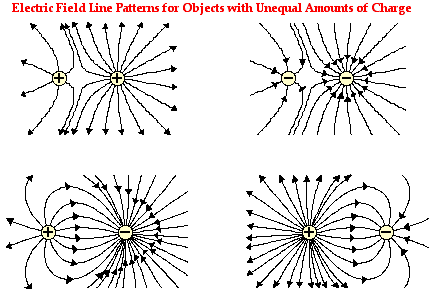
\includegraphics[scale=0.45]{fieldlines}
\caption{Representing Electric Field Lines}
\end{figure}
\end{frame}

\begin{frame}{Drawing Electric Field Lines}{}
  \begin{itemize}
	\item Number of lines drawn is proportional to magnitude of the charge
  \end{itemize}
\begin{figure}
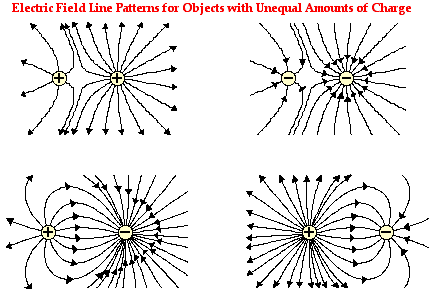
\includegraphics[scale=0.45]{fieldlines}
\caption{Representing Electric Field Lines}
\end{figure}
\end{frame}

\begin{frame}{Drawing Electric Field Lines}{}
  \begin{itemize}
	\item Field lines do not “cross” because the direction of E at a point is unique.
  \end{itemize}
\begin{figure}
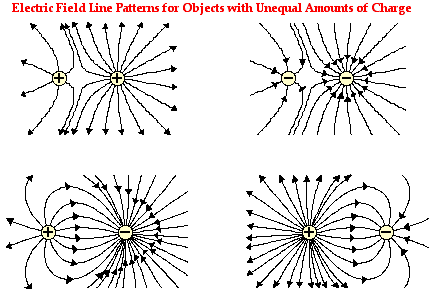
\includegraphics[scale=0.45]{fieldlines}
\caption{Representing Electric Field Lines}
\end{figure}
\end{frame}

\begin{frame}{Drawing Electric Field Lines}{}
  \begin{itemize}
	\item  At locations where electric field lines meet the surface of an object, the lines are perpendicular to the surface
  \end{itemize}
\begin{figure}
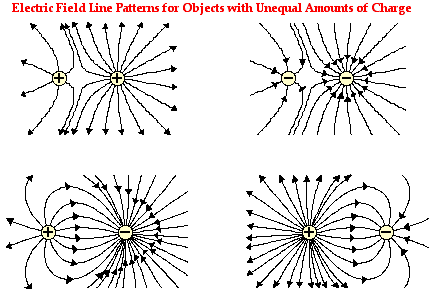
\includegraphics[scale=0.45]{fieldlines}
\caption{Representing Electric Field Lines}
\end{figure}
\end{frame}

	
\begin{frame}{Electric Field Lines as an Invisible Reality}{}
  \begin{itemize}
    \item Electric field lines are not real!
	\item The concept of an electric field arose as scientists attempted to explain the action-at-a-distance that occurs between charged objects
	\item First introduced by 19th century physicist Michael Faraday
	\item Rather than thinking in terms of one charge affecting another charge, Faraday used the concept of a field to propose that a charged object (or a massive object in the case of a gravitational field) affects the space that surrounds it
	\item  As another object enters that space, it becomes affected by the field established in that space
	\item Viewed in this manner, a charge is seen to interact with an electric field as opposed to with another charge
  \end{itemize}
\end{frame}

\begin{frame}{Are you still with us?}
Where do electrons play football? On an electric field!
\end{frame}

\begin{frame}{Force between Two Point Charges}
  \begin{block}{Couloumb's Law}
The magnitude of the electrical force acting between two point charges is proportional to the product of the magnitude of the charges and inversely proportional to the square of the distance between them.
\[F=\frac{1}{4\pi \epsilon_0} \cdot \frac{QQ\prime}{r^2} \]
  \end{block}
\end{frame}

\begin{frame}{Permittivity}{}
  \begin{itemize}
  \item Permittivity is the measure of the resistance that is encountered when forming an electric field in a medium. In other words, permittivity is a measure of how an electric field affects, and is affected by, a dielectric medium.
  \item \(\epsilon_0\) is equal to approximately \(8.85 \cdot 10^{-12}\) farad per meter \(Fm^{-1}\) in free space (a vacuum)
  \end{itemize}
\end{frame}

\begin{frame}{Principle of Superposition}
\begin{block}{Principle of Superposition (for electrical forces)}
The resultant force on any one of them equals to the vector sum of the forces exerted by the other individual charges.
\end{block}

Let's work out Example 2 together.
\end{frame}

\begin{frame}{Electric Field around a Point Charge}{}
  \begin{itemize}
  \item Recall Coulomb's Law
\[F=\frac{1}{4\pi \epsilon_0} \cdot \frac{Qq}{r^2} \]
\begin{block}{Electric Field Strength}
The magnitude of the electric field strength of a point charge \(Q\) at a distance \(r\) away from the field is
\[E=\frac{F}{q}\]
\[E=\frac{1}{4\pi \epsilon_0} \cdot \frac{Q}{r^2}\]
\end{block}
  \end{itemize}
\end{frame}

\begin{frame}{Electric Field around a Point Charge}{}
  \begin{itemize}
  \item Analogous to gravitational field strength
  \item Instead of \(g=\frac{F_g}{m}\), we now have \(E=\frac{F_E}{q}\)!
  \end{itemize}
\end{frame}

\begin{frame}{Electric Field around a Point Charge}{}
  \begin{itemize}
  \item \(E\) is a vector quantity, and its direction is at a point is given by the direction of the force experienced by a positive charge if it is placed at that point.
  \item The field is radial of a point charge. It is directed uniformly in all directions outward from the centre if \(Q\) is a positive charge and inward toward the centre if \(Q\) is a negative charge. At all points that are equal distance away from \(Q\) the magnitude of \(E\) is the same.
  \end{itemize}
\end{frame}

\begin{frame}{Principle of Superposition (for Electric Field)}{}
  \begin{itemize}
\begin{block}{Principle of Superposition (for Electric Field)}
The resultant electric field \(E\) at a point \(P\) in an electric field is the vector sum of the fields at \(P\) due to each point charge in the system.
\end{block}
  \item Very intuitive, right?
  \item Let's now work on Example 3 together.
  \end{itemize}
\end{frame}

\begin{frame}{Electric Potential}{}
  \begin{itemize}
\begin{block}{Definition of Electric Potential}
The electric potential V, at a point in an electric field, is defined as the work done per unit positive charge, by an external force, in moving a small test charge from infinity to that point in the electric field.
\[V=\frac{W}{q}\]
\end{block}
  \item SI unit of electric potential is \(JC^{-1}\) but it is more common to use the volt, \(V\)
  \end{itemize}
\end{frame}

\begin{frame}{Electric Potential}{}
Potential energy is the capacity for doing work which arises from position or configuration. In the electrical case, a charge will exert a force on any other charge and potential energy arises from any collection of charges. For example, if a positive charge Q is fixed at some point in space, any other positive charge which is brought close to it will experience a repulsive force and will therefore have potential energy.
\end{frame}

\begin{frame}{Potential due to a Point charge}{}
Electric potential in a field can arise due to a point charge Q, which is given by
\begin{block}{Electric Potential}
\[V=\frac{1}{4\pi \epsilon_0} \cdot \frac{Q}{r} \]
\end{block}
  \begin{itemize}
  \item The potential at a point can always be determined by
  \[V_{resultant} = V_1 + V_2 + V_3...\]
  \item Let's work on example 4 together.
  \end{itemize}
\end{frame}


\begin{frame}{Electric Potential Energy}{}
\begin{block}{Electric Potential Energy}
The electric potential energy, \(U\) of a charge at a point in an electric field is defined as the work done by an external agent in moving the charge from infinity to that point.
\end{block}
\end{frame}

\begin{frame}{Electric Potential Energy}{}
\begin{block}{Relationships between \(U\) and \(V\)}
\[U=qV\]
\end{block}
  \begin{itemize}
  \item Recall that potential energy in gravitational field is \(U=m\phi \)
  \item Notice any similarities?
  \end{itemize}
\end{frame}

\begin{frame}{Electric Potential Energy}{}
\begin{block}{Relationships between \(U\) and \(V\)}
Work done by the external agent in moving a charge Q from point A to point B in an electric field is given by
\[U_{A\to B}=U_B-U_A=Q(V_B-V_A)\]
\end{block}
Similar to gravitational potential energy, the electric potential energy is stored in a system of charges and not possessed by a single charge \(Q\).
\end{frame}

\begin{frame}{Electric Potential Energy}{}
  \begin{itemize}
  \item Work done in moving a charge from point A to point B, and 
  \item The change in potential energy is independent of the path taken
  \end{itemize}
\end{frame}

\begin{frame}{Potential Energy of a System of Two Point Charges}{}
  \begin{itemize}
  \item Given two charges \(Q_1\) and \(Q_2\) separated by a distance \(r\). \(Q_1\) sets up an electric field around the region and Q2 is in the electric field of \(Q_1\). Hence, 
  \item Potential of the electric field by Q1 at where Q2 is	 \[V=\frac{Q_1}{4\pi \epsilon_0 r}\]
  \item Multiplying both sides by \(Q_2\), we get the potential energy of the system, \(U\)
\begin{block}{Potential Energy Between Two Point Charges}
  \[U=Q_2V = \frac{Q_1Q_2}{4\pi \epsilon_0 r}\]
\end{block}
    \end{itemize}
\end{frame}

\begin{frame}{Potential Energy of a System of Two Point Charges}{}
Since any negative sign on the charge represents the direction, the magnitude can be found by ignoring the charge and including it afterwards when the magnitude of potential energy is obtained.
\end{frame}

\begin{frame}{Potential Energy of a System of Two or More Charges}{}
We will demonstrate the potential energy of a system with three charges
  \begin{itemize}
  \item Step One: Bring \(q_1\) from infinity to the point.  As there is no electric field initially in the region, work done \[W_1=0J\]
  \end{itemize}
\end{frame}

\begin{frame}{Potential Energy of a System of Two or More Charges}{}
  \begin{itemize}
  \item Step Two: Bring \(q_2\) from infinity to the point.  As \(q_1\) is already in place, it would have set up an electric field in the region and an external force will need to do work against the electrical force experienced by \(q_2\) due to its interaction with the field set up by \(q_1\). Hence, work done
  \[W_2=\frac{q_1 q_2}{4\pi \epsilon_0 r_{12}}\]
  \end{itemize}
\end{frame}

\begin{frame}{Potential Energy of a System of Two or More Charges}{}
  \begin{itemize}
  \item Step Three: We bring \(q_3\) from infinity to its position in the electric field.  Since, \(q_1\) and \(q_2\) are now in place, the electric field in the region is now due to \(q_1\) and \(q_2\), and the external force will need to do work against the force on \(q_3\) due to its interaction with the field set up by both \(q_2\) and \(q_3\). Hence, the work done in this process is
  \[W_3=\frac{q_1 q_3}{4\pi \epsilon_0 r_{13}} + \frac{q_2 q_3}{4\pi \epsilon_0 r_{23}}\]
  \item For more charges, use the same idea
  \end{itemize}
\end{frame}


\begin{frame}{Potential Energy of a System of Two or More Charges}{}
  \begin{itemize}
  \item Hence, the net potential energy of the system is the net work to assemble the system:
Potential energy of this system, \(U=W_{12} + W_{13} + W{23} \)
\[=\frac{q_1 q_2}{4\pi \epsilon_0 r_{12}} + \frac{q_1 q_3}{4\pi \epsilon_0 r_{13}} + \frac{q_2 q_3}{4\pi \epsilon_0 r_{23}}\]
  \item For more charges, use the same concept
  \end{itemize}
\end{frame}


\begin{frame}{Derivation of Electrical Force}{}
\[U=\int_{\infty}^r F_{ext}dr\]
\[\frac{dU}{dr}=F_{ext}\]
but \(F_E = -F_{ext}\)
\[F_E=-\frac{dU}{dr}\] 
\end{frame}

\begin{frame}{Electrical Force}{}
\begin{block}{Relation between Potential Energy and Electrical Force}
From here, we can see that:
\[F=-\frac{dU}{dr}\]
\end{block}
  \begin{itemize}
  \item Magnitude of force given by
\[F=\left|\frac{dU}{dr}\right(|\]
  \item The direction of the force on the charge is given by the negative (-) sign i.e. the force on the charge points towards a decreasing potential energy (towards the point that allows the charge to achieve a lower energy).
  \end{itemize}
\end{frame}

\begin{frame}{Potential Gradient}{}
\begin{block}{Relation between Potential Gradient and Electric Field Strength}
\[F=-\frac{dU}{dr}\]
\[qE=-\frac{dqV}{dr}\]
\[E=-\frac{dV}{dr}\]
\end{block}
  \begin{itemize}
  \item \(\frac{dV}{dr}\) is known as the potential gradient of the field.
  \end{itemize}
\end{frame}

\begin{frame}{Equipotential Lines or Surfaces}{}
\begin{definition}{}
An equipotential surface is a surface in which every point on the surface is at the same potential.
\end{definition}
\begin{figure}
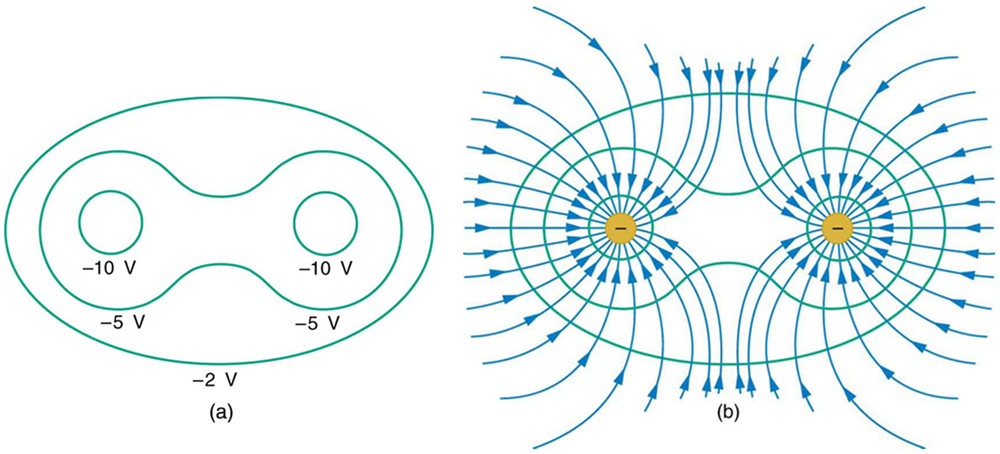
\includegraphics[scale=0.2]{equipotential}
\caption{Equipotential Lines}
\end{figure}
\end{frame}

\begin{frame}{Equipotential Lines or Surfaces}{}
\begin{itemize}
  \item Field strength: Spacing of equipotential lines
  \item Field lines and equipotential lines cut at right angles
  \item Field direction: Towards lower potential
  \end{itemize}
\begin{figure}
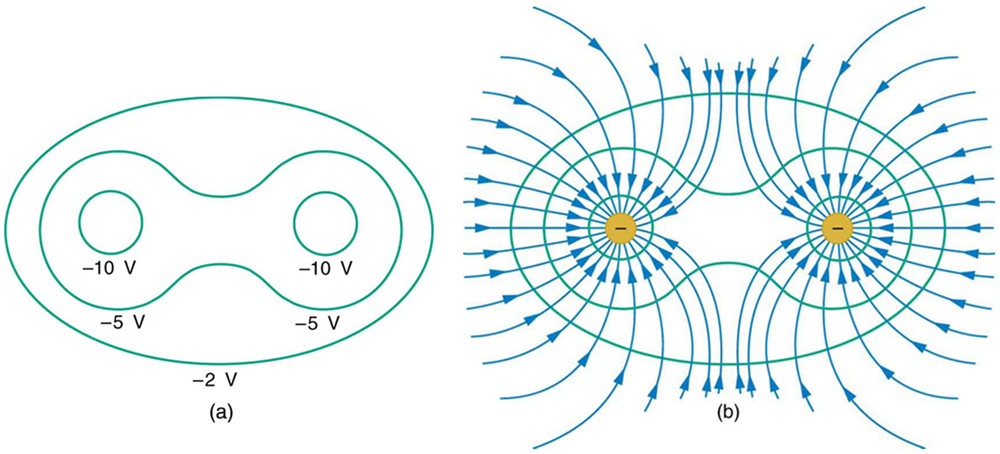
\includegraphics[scale=0.2]{equipotential}
\caption{Equipotential Lines}
\end{figure}
\end{frame}


\begin{frame}{Charges in Equilibrium on Conductors}{}
  \begin{itemize}
  \item Charged conductors that have reached electrostatic equilibrium share a variety of unusual characteristics. 
  \item One characteristic of a conductor at electrostatic equilibrium is that the electric field anywhere beneath the surface of a charged conductor is zero. 
  \item If an electric field did exist beneath the surface of a conductor (and inside of it), then the electric field would exert a force on all electrons that were present there. 
  \end{itemize}
\end{frame}

\begin{frame}{Charges in Equilibrium on Conductors}{}
  \begin{itemize}
  \item This net force would begin to accelerate and move these electrons. But objects at electrostatic equilibrium have no further motion of charge about the surface. So if this were to occur, then the original claim that the object was at electrostatic equilibrium would be a false claim.
  \item If the electrons within a conductor have assumed an equilibrium state, then the net force upon those electrons is zero. 
  \end{itemize}
\end{frame}

\begin{frame}{Charges in Equilibrium on Conductors}{}
  \begin{itemize}
   \item The electric field lines either begin or end upon a charge and in the case of a conductor, the charge exists solely upon its outer surface. 
  \item The lines extend from this surface outward, not inward. This of course presumes that our conductor does not surround a region of space where there was another charge.
  \end{itemize}
\end{frame}

\begin{frame}{Additional rules on drawing Electric Field/Equipotential Lines}{}
  \begin{enumerate}
   \item Electric field along the surface is zero
   \item The surface of a conductor is an equipotential surface
   \item The potential in the conductor is constant everywhere inside the conductor and equal to its value at the surface
   \item Electric field in the conductor is therefore zero. (No potential gradient) Hence, no field lines are drawn.
  \end{enumerate}
\end{frame}

\begin{frame}{Electric Field between Two Charged Parallel Plates}{}
  \begin{itemize}
	\item The charges on each plate are spread uniformly over the inside surface of each plate because of their mutual repulsion and the attraction by the opposite charges on the other plate.
	\item The lines of forces are straight, parallel to each other and equally spaced.
  \end{itemize}
\begin{figure}
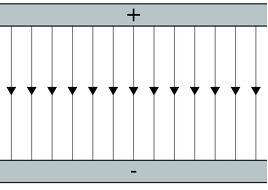
\includegraphics[scale=0.4]{parallelplates}
\caption{Electric Field between two parallel oppositely charged plates}
\end{figure}
\end{frame}

\begin{frame}{Electric Field between Two Charged Parallel Plates}{}
  \begin{itemize}
	\item The electric field in the space between the two plates is said to be uniform.
  \end{itemize}
  \begin{block}{Magnitude of Electric Field Strength}
\[E=\frac{V}{d}\]
\end{block}
\begin{figure}
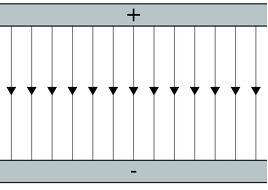
\includegraphics[scale=0.4]{parallelplates}
\caption{Electric Field between two parallel oppositely charged plates}
\end{figure}
\end{frame}

\begin{frame}{Motion of Charged Particles in a Uniform Electric Field}{}
  \begin{itemize}
	\item Consider a particle of mass \(m\), carrying charge \(q\) and placed in an uniform electric field \(E\).
	\item The field exerts a force \(qE\) on it, giving it an acceleration \(a\) in the direction of the force.
	\item By N2L, \(ma=qE\)
	\item Acceleration of the charge is therefore given by
	\[a=\frac{qE}{m} \]
	\item Note that in most questions, the mass is so small that the electric force overwhelms the gravitational force on the mass (weight). Hence the weight can be ignored.   
  \end{itemize}
\end{frame}


\begin{frame}{Gauss's Law}{}
\texttt{https://www.youtube.com/watch?v=QNIJC1emss8}
\begin{block}{Gauss's Law}
The net electric flux through any closed surface is equal to \(\frac{1}{\epsilon_0}\) times the net electric charge enclosed within that closed surface.
\end{block}
  \begin{itemize}
  \item It was formulated by Carl Friedrich Gauss in 1835, and finally published in 1867.
  \item It is one of the four Maxwell’s equations, forming the basis of classical electrodynamics.
  \item Gauss’s Law can be used to derive Coulomb’s Law, and vice versa.
  \end{itemize}
\end{frame}

\begin{frame}{Gauss's Law}{}
Integral form:
\[\oint_S {E_n dA = \frac{1}{{\varepsilon _0 }}} Q_{inside}\]
Differential form:
\[\nabla E=\frac{\rho}{\epsilon_0}=4\pi k\rho\]
  \begin{itemize}
  \item Its integral form is useful for calculating electric fields around charged objects.
  \item Its differential form is mathematically equivalent to its integral form.
  \item \(\nabla E\) is the divergence of the electric field, \(\epsilon_0\) is the electric constant, and \(\rho\) is the total electric charge density (charge per unit volume).
  \end{itemize}
\end{frame}

\section*{Summary}

\begin{frame}{Summary}
  \begin{itemize}
  \item The electric field is a field of force
  \item \(E=\frac{F}{q}\)
  \item Rules for drawing electric fields
  \item Coulomb's law
  \[F=\frac{1}{4\pi \epsilon_0} \cdot \frac{QQ\prime}{r^2} \]
  \item Electric Field
  \item Electric Potential
  \item Electric Potential Energy
  \item Potential Energy of a System of Two or More Point Charges
  \end{itemize}
\end{frame}

\begin{frame}{Summary}
  \begin{itemize}
  \item Potential Energy of a System of Two or More Point Charges
  \item Electrical Force
  \item Potential Gradient
  \item Equipotential Lines
  \item Charges in Equilibrium on Conductors
  \item Electric field between Parallel Charged Plates
  \item Motion of Charged Particles in an Uniform Electric Field
  \item Gauss's Law
  \end{itemize}
\end{frame}

\begin{frame}{End}
We have come to the end of our presentation. We hope you have enjoyed it.
\end{frame}
\end{document}


